\section{Testing}
\label{testing}

We measured the execution time and RAM usage of our three Mini-MAC implementations 
running on the Texas Instruments MSP430F5529 microcontroller. 
In speed and power this device is representative of vehicular ECUs.

\subsection{Purpose}
\label{purpose}

The purpose of our tests is to measure the time and space usage of our Mini-MAC, and more generally,
to evaluate the performance suitability of Mini-MAC for authenticating messages on the CAN bus.

\subsection{Methods}
\label{methods}

For each implementation we measured code size, memory usage, execution time, and bus utilization,
collecting for each implementation metrics from 1000 inputs of various typical sizes.  

%["various sizes" is rather vague]

We measured code size and RAM usage at complile time using 
the Texas Instruments Code Composer v6.

%% is there a difference between compiled metrics and flashed metrics? If not, I don't understand your comment:
%% provides values for both after code is compiled and flashed to the MSP430 hardware.
%% Are you correct to assume execution RAM pace is same as compiled RAM space?

We measured execution time using a counter register on the MSP430, 
whose 32kHz clock provides timing values to approximate millisecond accuracy. 
There may be a +/-0.03~ms inaccuracy in each reading due to the
time it takes to read the counter.

%% ?! if the clock is accurate to 1 ms, why are you talking about secondary 0.03 ms errors?
%% How can you know the error is only 0.03 ms if the timing accurance is 1 ms?
%% Maybe delete the last sentence.

We collected statistics on message traffic from a 2010 Toyota Prius with a CAN-bus sniffer program 
based on an Arudiuno Uno platform and connected via an OBD-II CAN transceiver shield.

\subsection{Results}
\label{results}

Tables~\ref{tab-traffic}, \ref{tab-overhead}, \ref{tab-time}
and Figures~\ref{fig-execution}, \ref{fig-code}, \ref{fig-ram}
summarize our results.
Throughout, ``B''~denotes bytes, ``b''~denotes bits, and ``ms''~denotes milliseconds.

[need to enhance fig captions]

% there was an analysis par here that I moved to analysis section
	
	\begin{table}
	\centering
	\caption{MAC Bus Traffic Addition}
	\label{tab-traffic}
	\vspace{8pt}
	\begin{tabular}{l|c}%
	\bfseries Function & \bfseries Add. Traffic (b) \\\hline \csvreader[late after line=\\]%
		{tables/bus_addition.csv}{function=\function,at=\at}%
		{\function & \at}%
	\end{tabular}
	\end{table}

	\begin{table*}	
	\centering	
	\caption{Mini-MAC Overhead Relative to HMAC}
	\label{tab-overhead}
	\vspace{8pt}
	\begin{tabular}{l|c|c|c}%
	\bfseries Hash & \bfseries Code Size (B) & \bfseries RAM Use (B) & \bfseries Execution Time (ms)\\\hline \csvreader[late after line=\\]%
		{tables/overhead.csv}{hash=\hash,code_size=\code_size,ram_size=\ram_size,exec_time=\exec_time}% 
		{\hash & \code_size & \ram_size & \exec_time}%
	\end{tabular}
	\end{table*}
	
	\begin{table}
	\centering
	\caption{Approximate Execution Time of Mini-MAC Construction}
	\label{tab-time}
	\vspace{8pt}
	\begin{tabular}{ @{}l | S[table-format=2.1]  @{}}
		%\toprule
		\hspace{2pt}\textbf{Hash} & {\textbf{Exec. Time (ms)}} \\
		\hline 
		\hspace{2pt}MD5 & 7.5 \\
		\hspace{2pt}SHA1 & 28.0 \\
		\hspace{2pt}SHA2 & 69.6 \\ 
		%\bottomrule
	\end{tabular}	
	\end{table}
	
	\begin{figure}
		\centering
		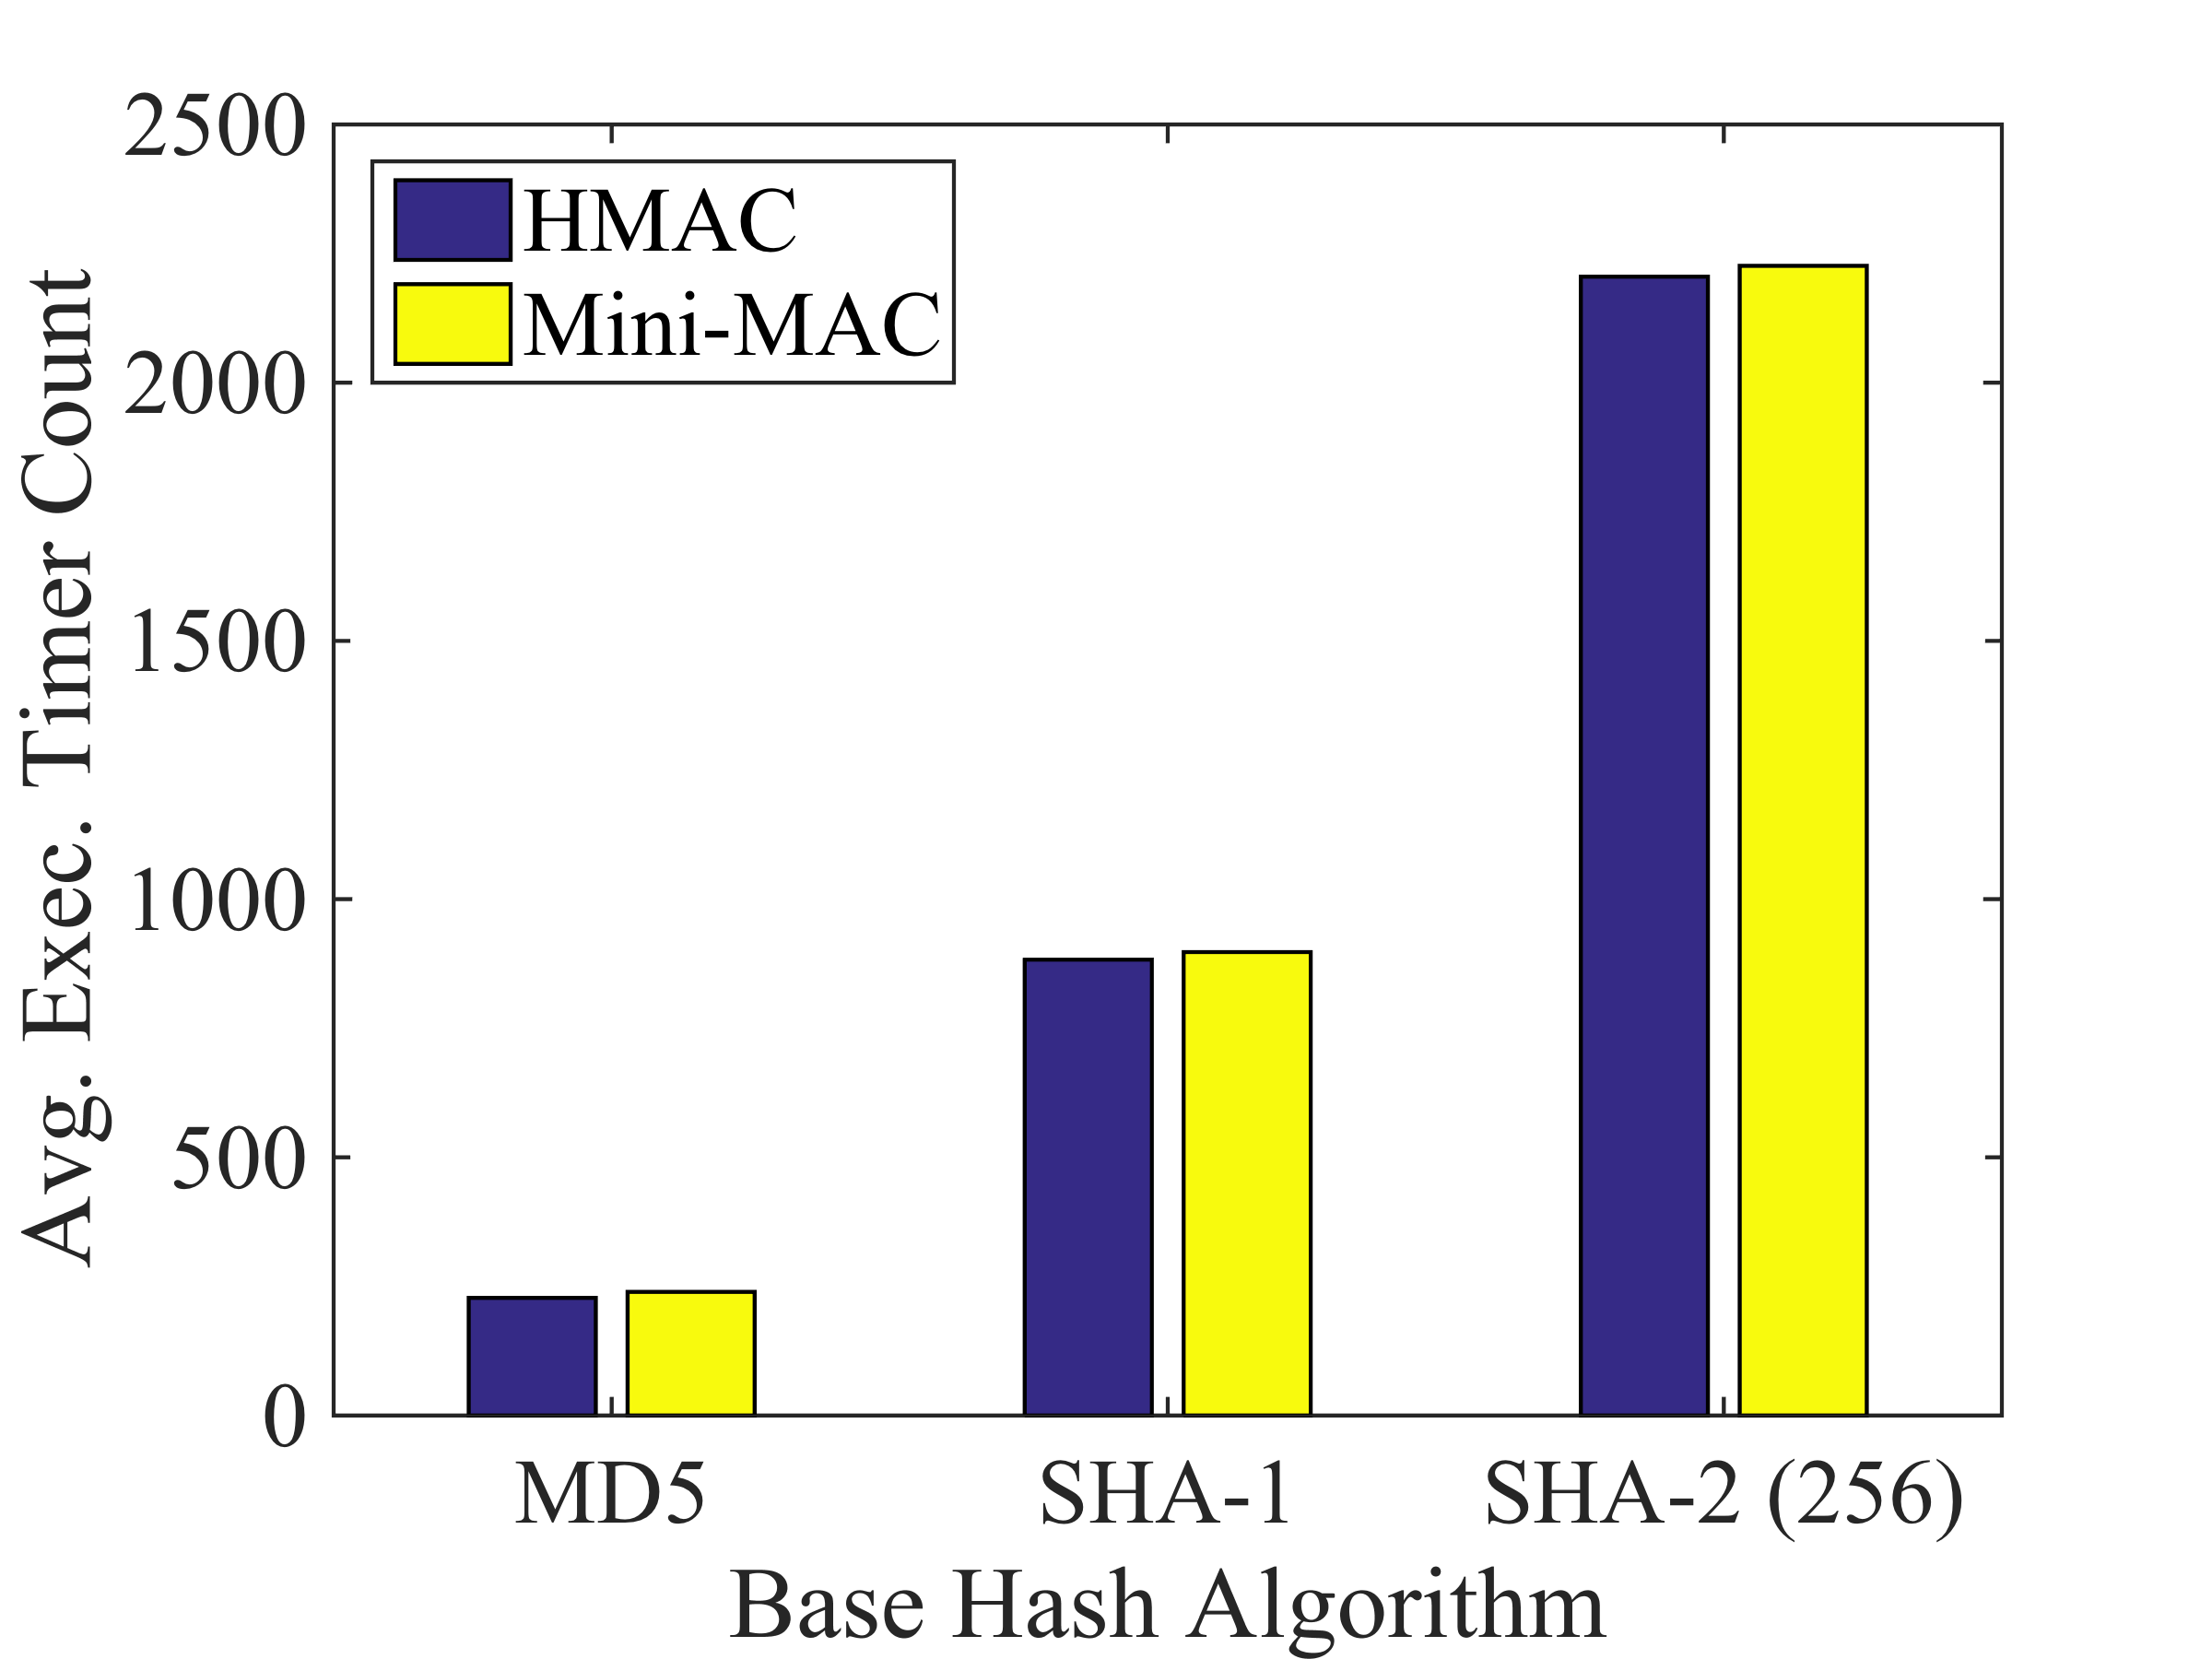
\includegraphics[width=\columnwidth]{figures/exec_cycles.png}
		\caption{Execution Time Comparison of Mini-MAC Construction}
		\label{fig-execution}
	\end{figure}
	
	\begin{figure}
		\centering
		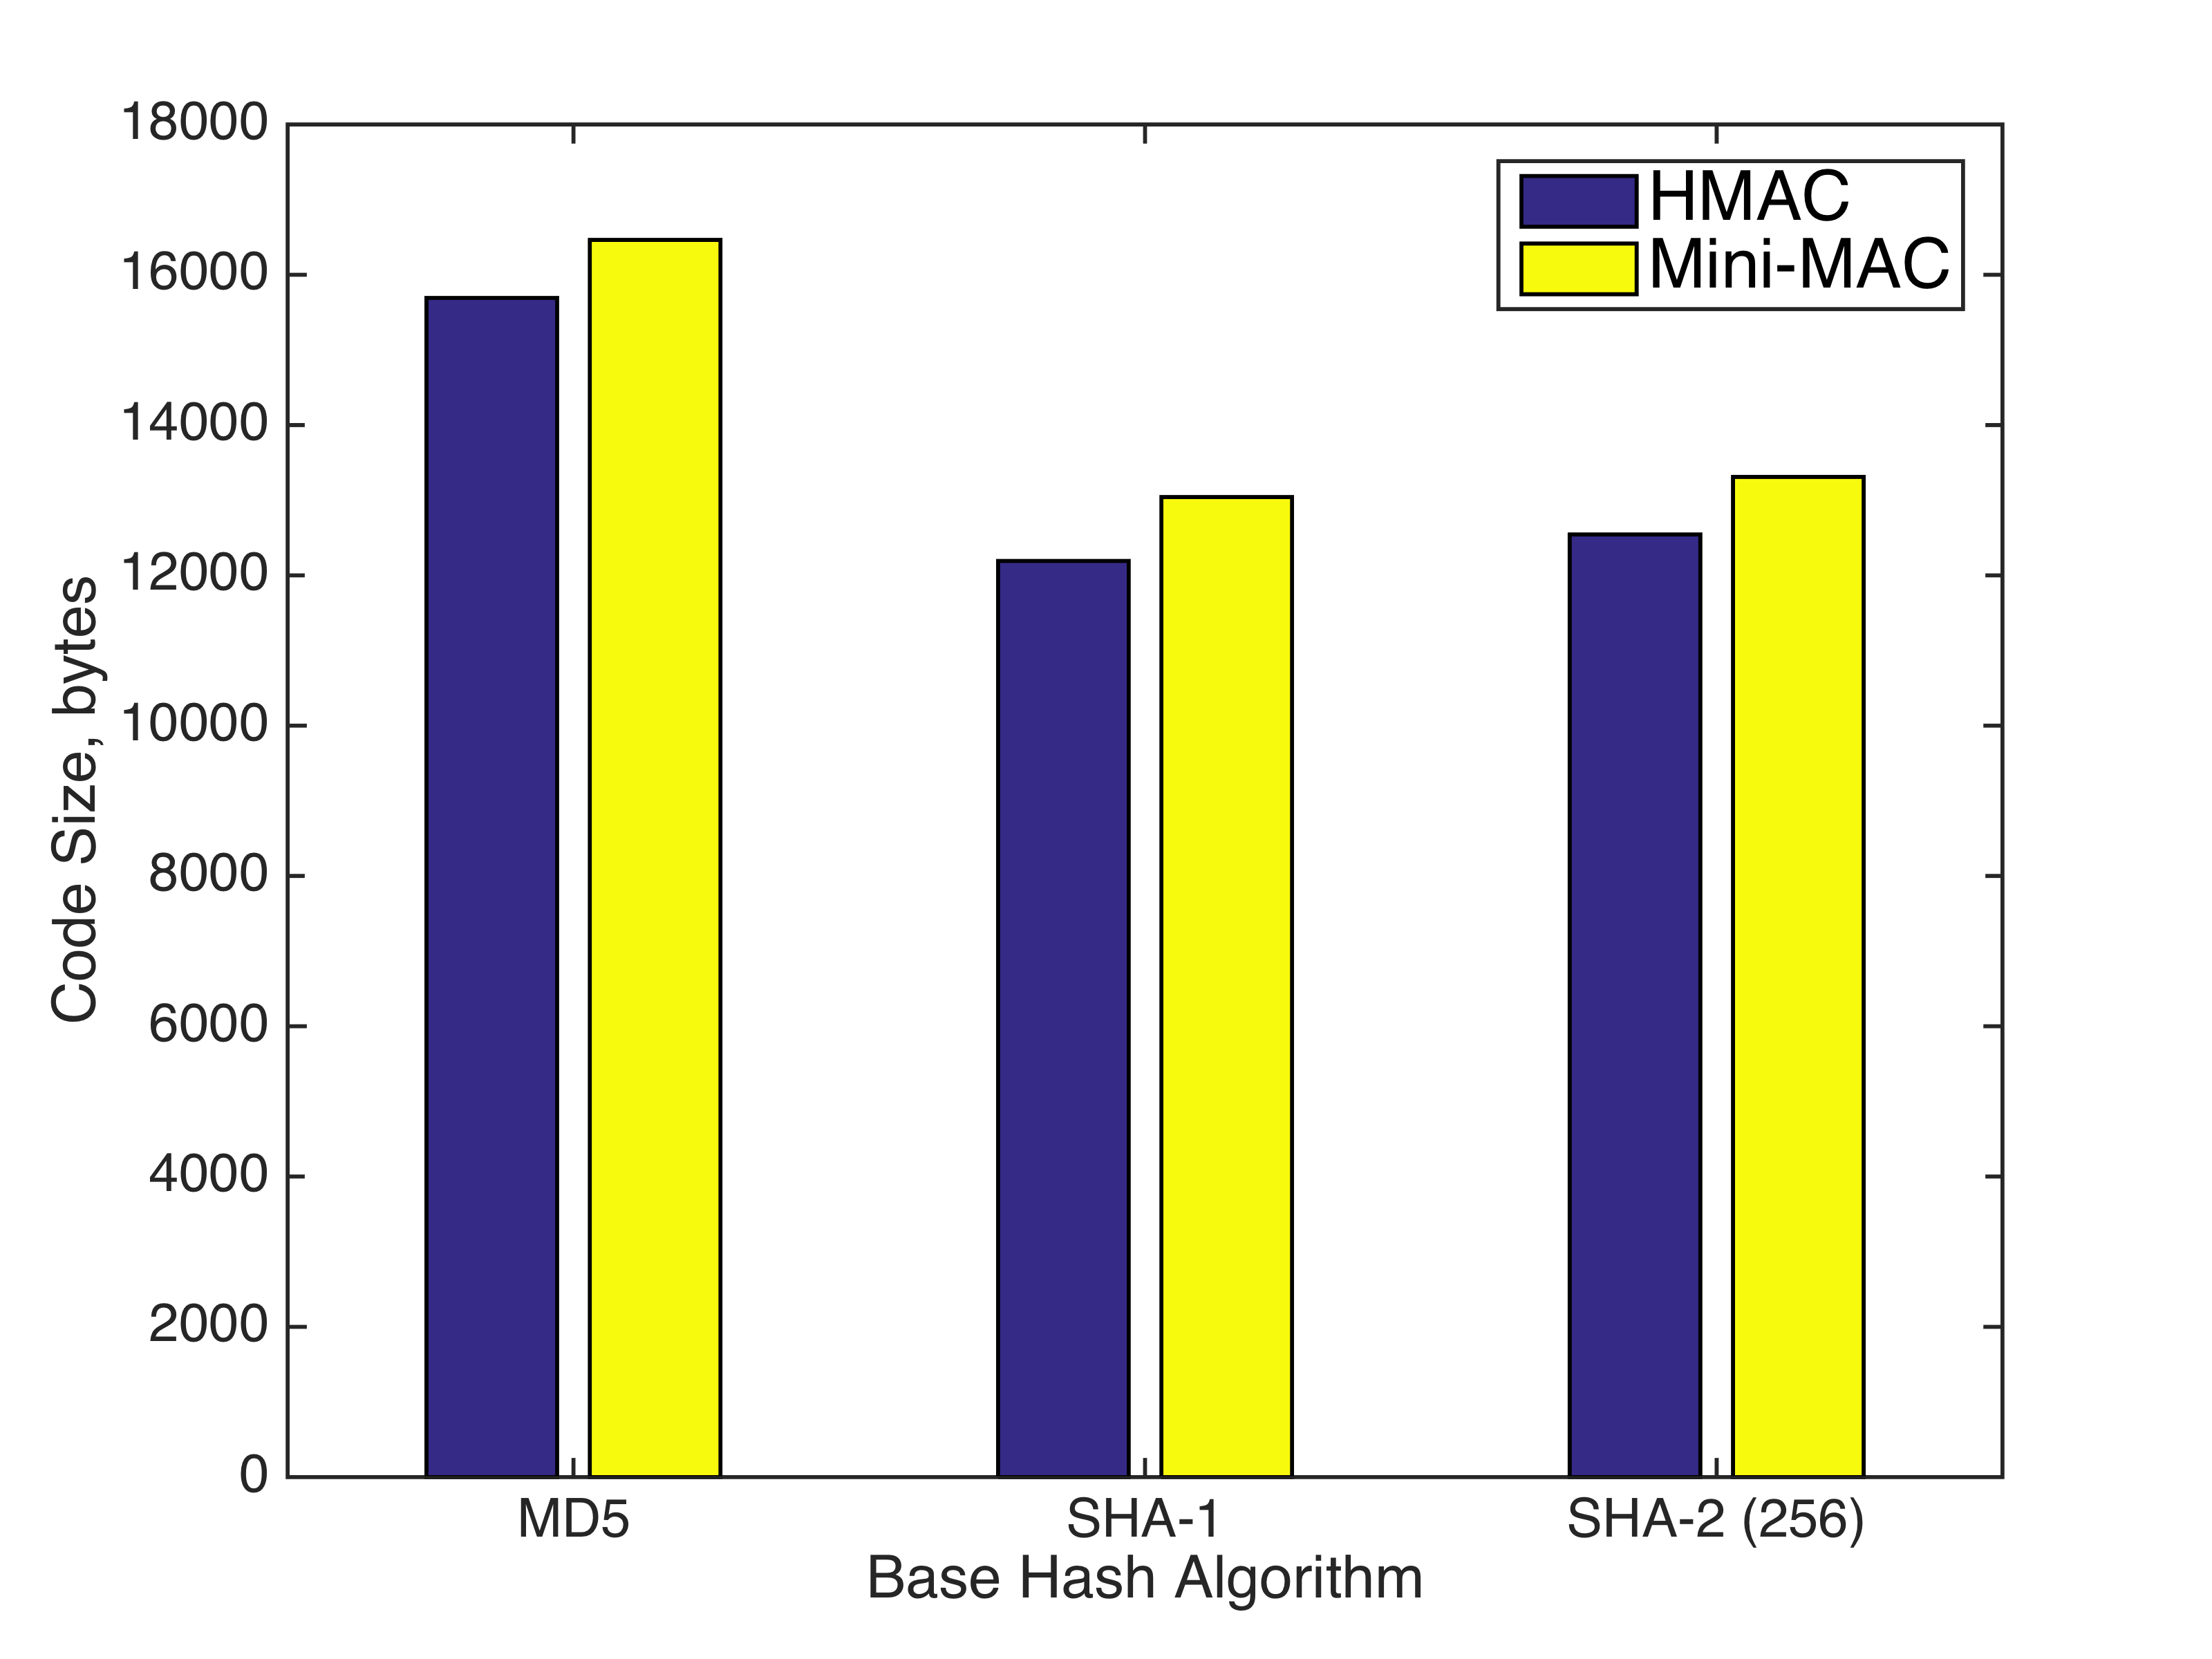
\includegraphics[width=\columnwidth]{figures/code_size.png}
		\caption{Code Size Comparison of Mini-MAC Code}
		\label{fig-code}
	\end{figure}
	
	\begin{figure}
		\centering
		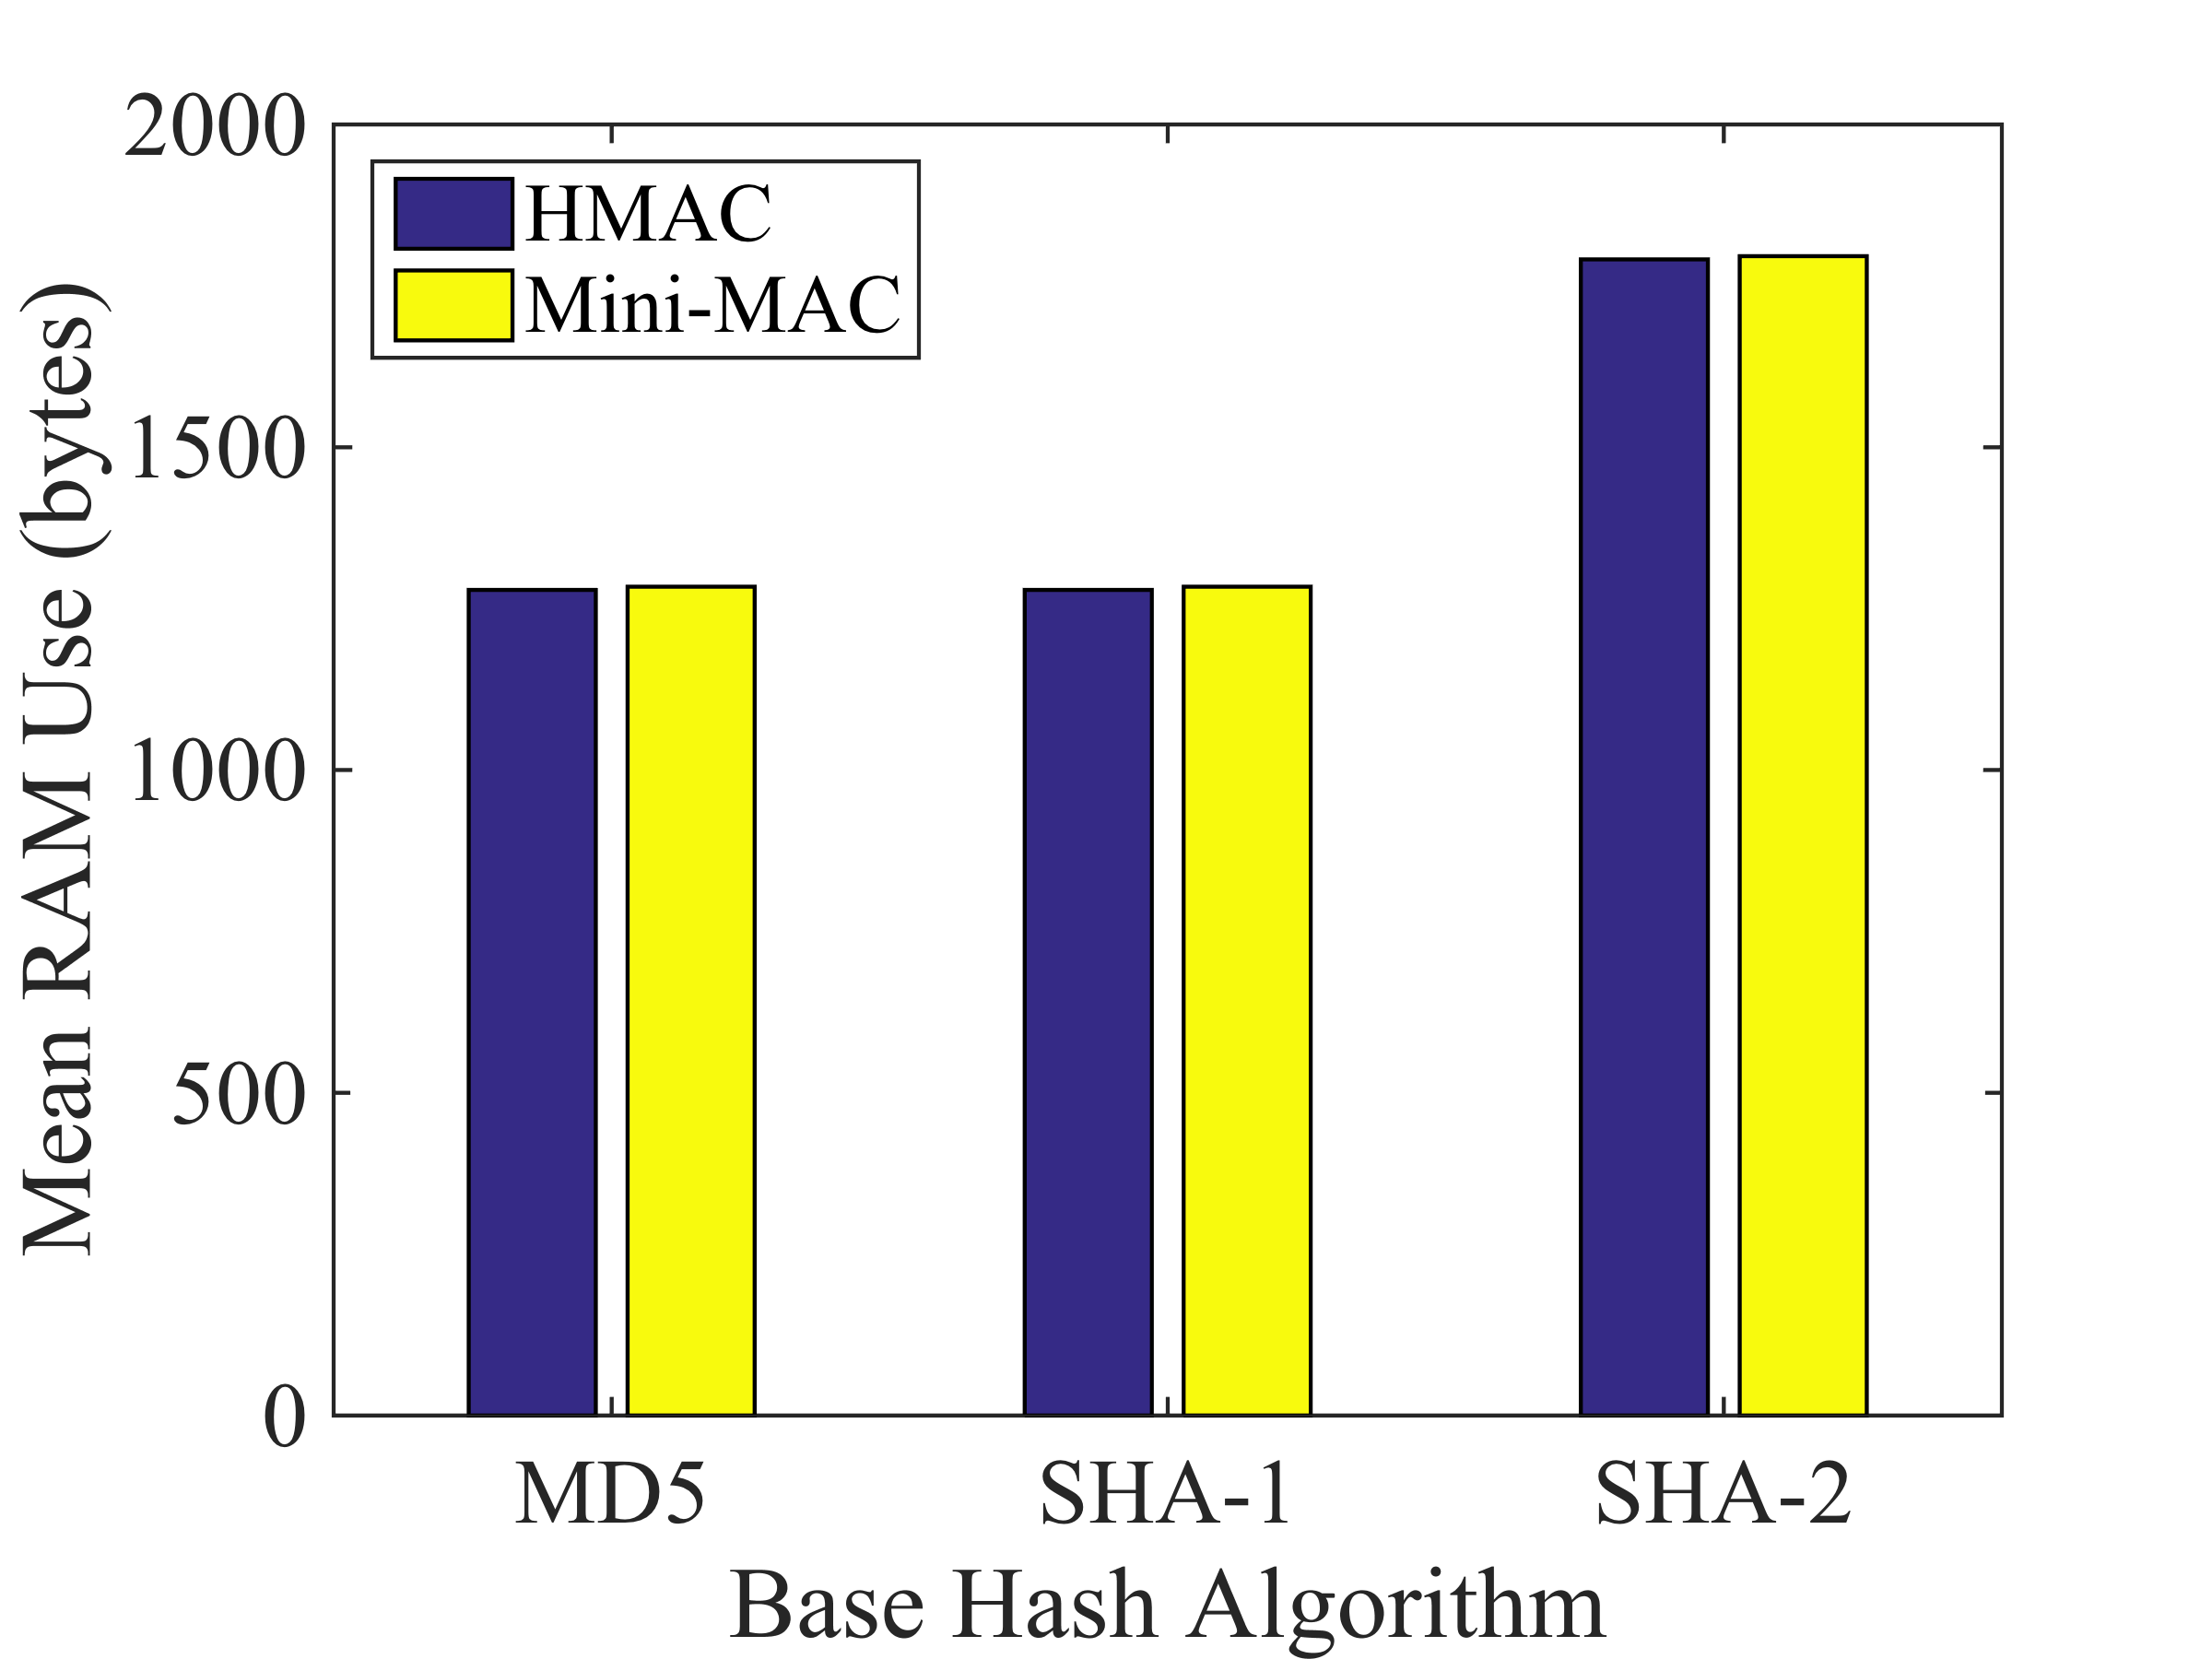
\includegraphics[width=\columnwidth]{figures/ram_usage.png}
		\caption{RAM Usage Comparison of Mini-MAC Code}
		\label{fig-ram}
	\end{figure}
	